% !TeX root = ../../main.tex
\subsection{Stress test and model boundary: ordered-bin FACS}

The Waterbear study supplies a complementary continuous-phenotype benchmark
with unusually useful validation \citep{pimentel2024waterbear}.  GSE242880
contains a pooled CRISPR screen of IL2RA protein abundance in primary human
T cells, from the regulatory-network study of \citet{freimer2022il2ra}, which
is also the source of the individually validated regulators used below.  Its low-coverage, high-MOI arm has four ordered FACS bins for each
of three donors, 6,000 guides targeting 1,350 genes or negative controls, and
26 regulators whose direction was confirmed by individual knockout and flow
cytometry.  Because these are primary donor cells rather than a cancer cell
line, this benchmark is not driven by tumor copy-number artifacts.

We assigned the four bins latent marker locations equal to the conditional
means of standard-normal intervals with the prespecified bin masses
$(0.2,0.3,0.3,0.2)$.  Beta-binomial regression used all 12 libraries with a
marker slope and donor indicators.  Official MAGeCK-MLE received the same
model space; its marker score was affinely mapped to zero--one because the
MAGeCK initializer requires a reference row with all non-intercept entries
zero.  We also fitted two outer-bin ablations and ran the paper's native
\texttt{mageck test} comparison of Q1 with Q4.

This design exposes a limitation of applying independent-library regression
to sorted data.  The four bins from one donor partition one cell pool and are
therefore negatively correlated, while the beta-binomial fit treats their
margins separately.  Among 593 non-targeting guides, the raw all-bin
beta-binomial $p<0.05$ frequency is 0.133.  We therefore added the
prespecified negative-control calibration implemented by
\texttt{bb\_calibrate\_controls()}: the empirical 95th percentile of absolute
control $t$ statistics is matched to the $t_8$ two-sided 0.05 cutoff, with
scales below one prohibited.  The estimated scale is 1.357; after calibration,
the non-targeting frequency is 0.049.  Estimates and the $t$ reference are
retained, while raw and calibrated inferential columns are both saved.

\begin{table}[ht]
\centering
\caption{GSE242880 low-coverage, high-MOI IL2RA FACS benchmark.  Recovery
uses each method's reported 0.10 discovery threshold and the independently
validated direction.  BARCS and MAGeCK use adjusted
$p$-values; Waterbear uses posterior inclusion probability above 0.90.
The non-targeting column is guide-level.  Waterbear and MAUDE values are
reported by the study and were not rerun.  The highest validated recovery and
the available non-targeting rate closest to 0.05 are highlighted.}
\label{tab:waterbear}
\small
\setlength{\tabcolsep}{4pt}
\begin{tabular}{lrrr}
\toprule
Method & Discoveries & Validated recovery & NTC $p<0.05$\\
\midrule
\methodswatch{barcsblue} BARCS, four bins + controls &
  49 & 22/26 & \textcolor{barcsblue}{\textbf{0.049}}\\
\methodswatch{barcsblue} BARCS, four bins raw & 127 & 23/26 & 0.133\\
\methodswatch{mageckorange} Official MAGeCK-MLE, four bins &
  72 & 17/26 & ---\\
\methodswatch{barcsblue} BARCS, outer bins & 34 & 18/26 & 0.064\\
\methodswatch{mageckorange} Official MAGeCK test, outer bins &
  32 & 18/26 & ---\\
\methodswatch{waterbearpurple} Waterbear, four bins (reported) &
  79 & 24/26 & ---\\
\methodswatch{maudered} MAUDE, four bins (reported) &
  406 & \textcolor{maudered}{\textbf{25/26}} & ---\\
\bottomrule
\end{tabular}
\end{table}

The calibrated four-bin BARCS result recovers four more
validated regulators than all-bin MAGeCK-MLE while making 23 fewer calls.  It
is two regulators behind the reported Waterbear result and three behind MAUDE.
The raw 23/26 BARCS result is not the primary claim because
its negative controls reveal inflation.  MAUDE's 25/26 recovery is also not
evidence of superior specificity: it calls 406 of 1,350 genes, and the
Waterbear study found poor MAUDE calibration in simulations
\citep{pimentel2024waterbear,deboer2020maude}.  Across all 1,350 genes,
uncalibrated BARCS and MAGeCK-MLE all-bin effects have
Spearman correlation 0.917, so the recovery difference is not caused by
globally incompatible directions.  All 26 validation effects have the
expected sign under each independently rerun method.

The follow-up table contains more information than the 26-positive subset.
Thirty-three candidates were tested individually: 26 had a concordant IL2RA
effect and seven did not validate.  Restricting evaluation to these measured
labels avoids the incorrect assumption that every other screen gene is a false
positive.  Table~\ref{tab:waterbearpanel} reports threshold and ranking metrics
for the five methods rerun here.

\begin{table}[ht]
\centering
\caption{Classification in the selected 33-gene experimental follow-up panel
(26 concordant positives and seven non-validating candidates).  This panel is
small and was selected from a previous screen, so the metrics are supporting
evidence rather than unbiased genome-wide performance estimates.  Higher is
better for every metric; column maxima are highlighted.}
\label{tab:waterbearpanel}
\small
\setlength{\tabcolsep}{4pt}
\begin{tabular}{lrrrrr}
\toprule
Method & F1 & MCC & Balanced accuracy & AUROC & Avg. precision\\
\midrule
\methodswatch{barcsblue} BARCS, four bins + controls
  & \textcolor{barcsblue}{\textbf{0.863}}
  & \textcolor{barcsblue}{\textbf{0.398}}
  & \textcolor{barcsblue}{\textbf{0.709}} & 0.808 & 0.945\\
\methodswatch{barcsblue} BARCS, four bins raw
  & 0.852 & 0.194 & 0.585
  & \textcolor{barcsblue}{\textbf{0.819}}
  & \textcolor{barcsblue}{\textbf{0.950}}\\
\methodswatch{mageckorange} Official MAGeCK-MLE, four bins
  & 0.723 & 0.070 & 0.541 & 0.626 & 0.872\\
\methodswatch{barcsblue} BARCS, outer bins
  & 0.783 & 0.340 & 0.703 & 0.714 & 0.913\\
\methodswatch{mageckorange} Official MAGeCK test, outer bins
  & 0.766 & 0.224 & 0.632 & 0.703 & 0.906\\
\bottomrule
\end{tabular}
\end{table}

The raw four-bin model has the strongest rank metrics, which indicates that the
continuous trend is extracting useful signal.  Control calibration changes the
decision boundary rather than the estimated effects and produces the best F1,
Matthews correlation, and balanced accuracy in the validation panel.  That
combination is the central evidence for BARCS here:
continuous-bin ranking gains are retained while explicit null guides prevent
the extra calls from being mistaken for confidence.

This benchmark is stronger than a rank-correlation-only comparison because it
contains directionally validated biology and hundreds of explicit null
guides.  It is not an unbiased precision experiment: the 26 genes were chosen
for follow-up from an earlier screen, and unvalidated genes cannot simply be
called false positives.  Nor does it overturn Waterbear's modeling advantage.
Waterbear represents the joint multinomial bin structure, uncertain cutoffs,
guide-to-gene hierarchy, and sparse effects; BARCS supplies
a much faster transparent trend test but needs negative controls here to
diagnose and scale inference under a violated independence assumption.  The deposited paper reports
24/26 for Waterbear and 17/26 for MAGeCK; the independent current
\texttt{mageck test} rerun gives 18/26, a one-gene implementation-level
difference.

These results separate three meanings of ``better.''  First, ranking quality
asks whether validated regulators move toward the top; the raw four-bin model
performs strongly by AUROC and average precision.  Second, decision quality
asks whether a prespecified threshold balances recovery and false calls; the
control-calibrated model leads the rerun methods by F1 and Matthews
correlation.  Third, likelihood fidelity asks whether the sampling dependence
is represented; Waterbear wins that design question because it models all bins
from a donor jointly.  The case for BARCS here rests on its performance on the first two questions
using a simple general-purpose model, together with the control diagnostic that
exposes the third.

\paragraph{MAUDE's own control calibration.}
MAUDE's reported 25/26 recovery is the highest in Table~\ref{tab:waterbear}, and
the non-targeting column is empty for it, so we measured that directly.  MAUDE
consumes non-targeting guides to build its empirical null, which means its
calibration cannot be read off the same guides it was given: those scores are
centred by construction, and all 593 return $p>0.2$.  We therefore split the
control set, declared half to MAUDE as its negative control, and relabelled the
other half so that each held-out guide is scored as its own element.  A held-out
non-targeting guide has no effect, so the rate at which it is called measures the
realised error rate against the nominal one.

Across 891 held-out control tests MAUDE runs at roughly twice its nominal rate
at every threshold: observed 0.021 at a nominal 0.01, 0.095 at 0.05, 0.190 at
0.10, and 0.377 at 0.20, for ratios of 2.13, 1.91, 1.90 and 1.89.  This
reproduces on experimental controls the poor MAUDE calibration that the
Waterbear study reported from simulation \citep{pimentel2024waterbear}, and it
places the 406 calls and 25/26 recovery in context: the recovery is real, and so
is the error rate that buys it.

One scope limit matters here.  MAUDE requires an unsorted reference sample, and
the low-coverage, high-MOI arm analysed above provides only the four sorted
bins, so this calibration was measured on the high-coverage, high-MOI arm, which
deposits a GFP unsorted sample per donor.  It is therefore not the same arm as
the BARCS figure of 0.049 and the two should not be subtracted; what transfers
between arms is the direction and magnitude of the inflation, not the digit.

The published Waterbear and MAUDE aggregates cannot be assigned validation-
panel F1 or Matthews correlation without their gene-level calls for all seven
non-validating candidates.  Reporting 24/26 or 25/26 as if it were complete
accuracy would therefore mix sensitivity with an unknown precision.  We retain
those values as positive-control recovery references and restrict
classification metrics to the methods rerun from complete outputs.

\begin{figure}[ht]
\centering
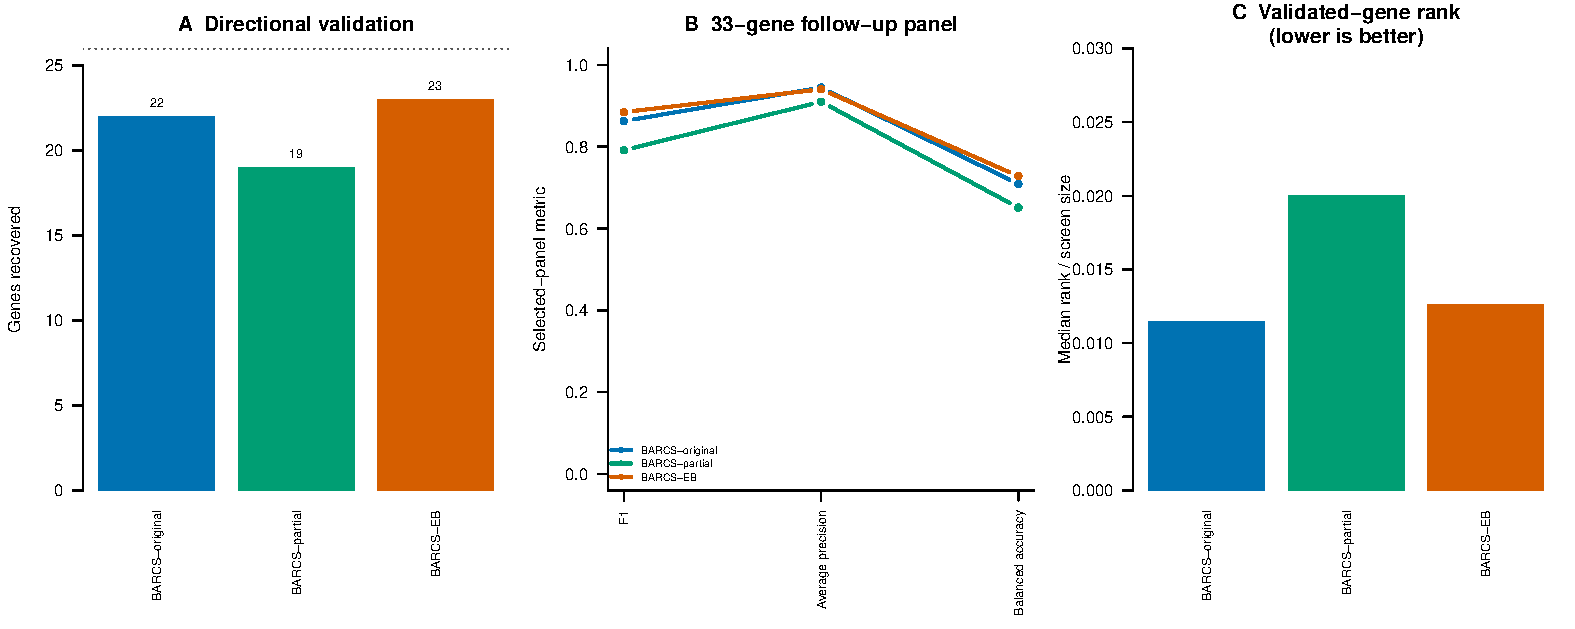
\includegraphics[width=\textwidth]{figures/waterbear_facs_benchmark.pdf}
\caption{Ordered-bin IL2RA FACS benchmark.  (A) Positive-control recovery for
all methods.  (B) F1 in the selected 33-gene panel for methods rerun here.
(C) All-bin BARCS and MAGeCK-MLE effects, with validated genes highlighted.
(D) Non-targeting-guide empirical null curves, showing the correction of raw
all-bin inflation.}
\label{fig:waterbear}
\end{figure}
\clearpage
